\documentclass[11pt]{report}
\usepackage{fullpage}
\usepackage{lingmacros}
\usepackage{tree-dvips}
\usepackage{minted}
\usepackage{graphicx}
\usepackage{hyperref}
\usepackage{keystroke}
\usepackage{url}
\hypersetup{
    colorlinks=true,
    linkcolor=blue,
    filecolor=magenta,      
    urlcolor=cyan,
    pdftitle={GPU Setup Guide},
    pdfpagemode=FullScreen,
    }
\graphicspath{{./images/}}



\begin{document}
    
\title{APSC 258: Training CNN with your computers GPU}
\author{Andre Cox}


\maketitle
\tableofcontents

\chapter{Introduction}
\section{The Problem}
In APSC 258 we have been using Google Colab to train our Convolutional Neural Networks. 
This is a great tool however recent versions of Colab have limited the GPU compute time.
This is a problem for us as we have a lot of data to train our CNN with. 
\section{The Solution}
However the solution to this problem is simple. We can use the dedicated GPU in your system to train your network.
Unfortunately only Nvidia GPUs are supported at this time. If you do not have a Nvidia GPU you could use an alternative to Colab such as \href{https://www.kaggle.com/}{Kaggle}. 
\section{Prerequisites}
Before we begin we need to check if your system has a Nvidia GPU.
To do this follow the steps below. Please note this only works on windows 10 and 11.
\begin{itemize}
    \item Enter the keyboard shortcut \Ctrl + \Shift + \Esc %show figure 1 
    \begin{center}
        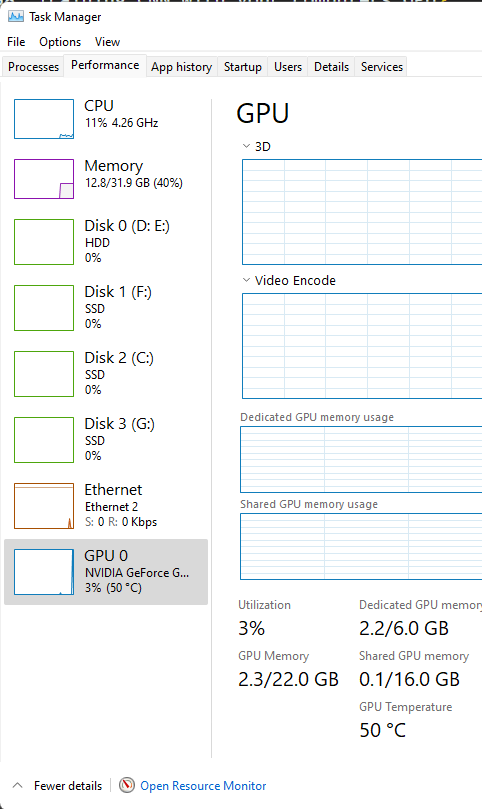
\includegraphics[width=0.5\textwidth]{taskmng.png}
    \end{center}
    You should see the task manager window. Select Peformance tab and then note if the GPU is a Nvidia GPU.
    \item If this is a Nvidia GPU then you can continue.
    \item If you have installed Anaconda or Python It is recommended that you uninstall these first before continuing.
    \item You can do this through "add or remove programs" in Windows 10/11.
\end{itemize}

\chapter{Dependencies}
\section{Deep Learning Libraries}
Pay attention to the version numbers, If these are incorrect this will not work. The correct versions have been linked for your convenience.
\begin{itemize}
    \item First we need to install \href{https://developer.nvidia.com/cuda-11.2.2-download-archive?target_os=Windows&target_arch=x86_64&target_version=10&target_type=exenetwork}{Cuda Toolkit 11.2.2}. IMPORTANT when installing this make sure you click "Custom (Advanced)" and deselect everything except "Development" and "Runtime".
    \item Next we need \href{https://developer.nvidia.com/compute/machine-learning/cudnn/secure/8.1.0.77/11.2_20210127/cudnn-11.2-windows-x64-v8.1.0.77.zip}{CUDNN 11.2 - 8.1.0.77}. You will need a developer account which you can create.
    \item Now Unzip the CUDNN zip file.
    \item Inside there should be 3 folders called bin, lib and include.
    \item Now open up Windows file explorer and paste in \begin{minted}[breaklines]{bash}
        C:/Program Files/NVIDIA GPU Computing Toolkit/CUDA/v11.2 
    \end{minted} 
    to the top bar.
    \item To finish installing CUDNN drag and drop lib, bin, and include folders into the 
    \begin{minted}[breaklines]{bash}
    C:/Program Files/NVIDIA GPU Computing Toolkit/CUDA/v11.2 folder.
    \end{minted}
    \item If any dialog boxes appear select yes.
\end{itemize}

\section{Development Dependencies}
We will be using winget to install our dependencies easily and quickly.
\begin{itemize}
    \item Open a new terminal by typing "CMD" in the search bar and selecting the first option.
    \item Install a specific version of python using 
    \begin{minted}[breaklines]{bash}
        winget install python3 -v 3.9.6150.0
    \end{minted}
    \item You may need to restart your computer now.
    \item Reopen the terminal and install your dependencies using 
    \begin{minted}[breaklines]{bash}
        pip install tensorflow keras numpy matplotlib pandas scipy pickle imgaug
    \end{minted}
    \item To install a Jupyter Notebook editor use 
    \begin{minted}[breaklines]{bash}
        winget install vscode
    \end{minted}
    \item Restart your computer.
    \item In your search bar you should now have a new program for working with .ipynb files.
    \begin{center}
    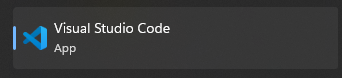
\includegraphics{vscode.png}
    \end{center}
    \item When opening an ipynb file vscode will let you know that there are extensions to help with these files. Allow these extensions to be installed.
    \item You're all finished! Now let's check if everything worked.
\end{itemize}
        

\chapter{Testing your GPU}
We can create a new ipynb file to test if your GPU is working. Paste this code into a Jupyter Notebook Cell and execute it. 
\begin{minted}[breaklines]{python}
import tensorflow as tf
device_name = tf.test.gpu_device_name()
if device_name != '/device:GPU:0':
  raise SystemError('GPU device not found')
print('Found GPU at: {}'.format(device_name))
\end{minted}

You should see this output.
\begin{center}
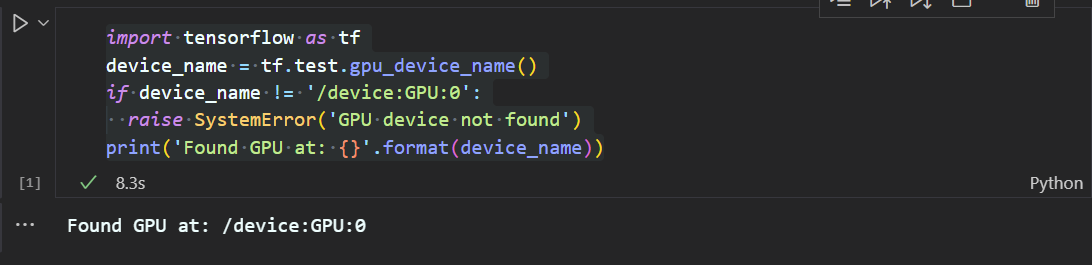
\includegraphics[width=1\textwidth]{gputest.png}
\end{center}

\section{Finishing Up}
Congratulations you have completed the installation of your GPU. You can now begin to train your CNN.
\begin{center}
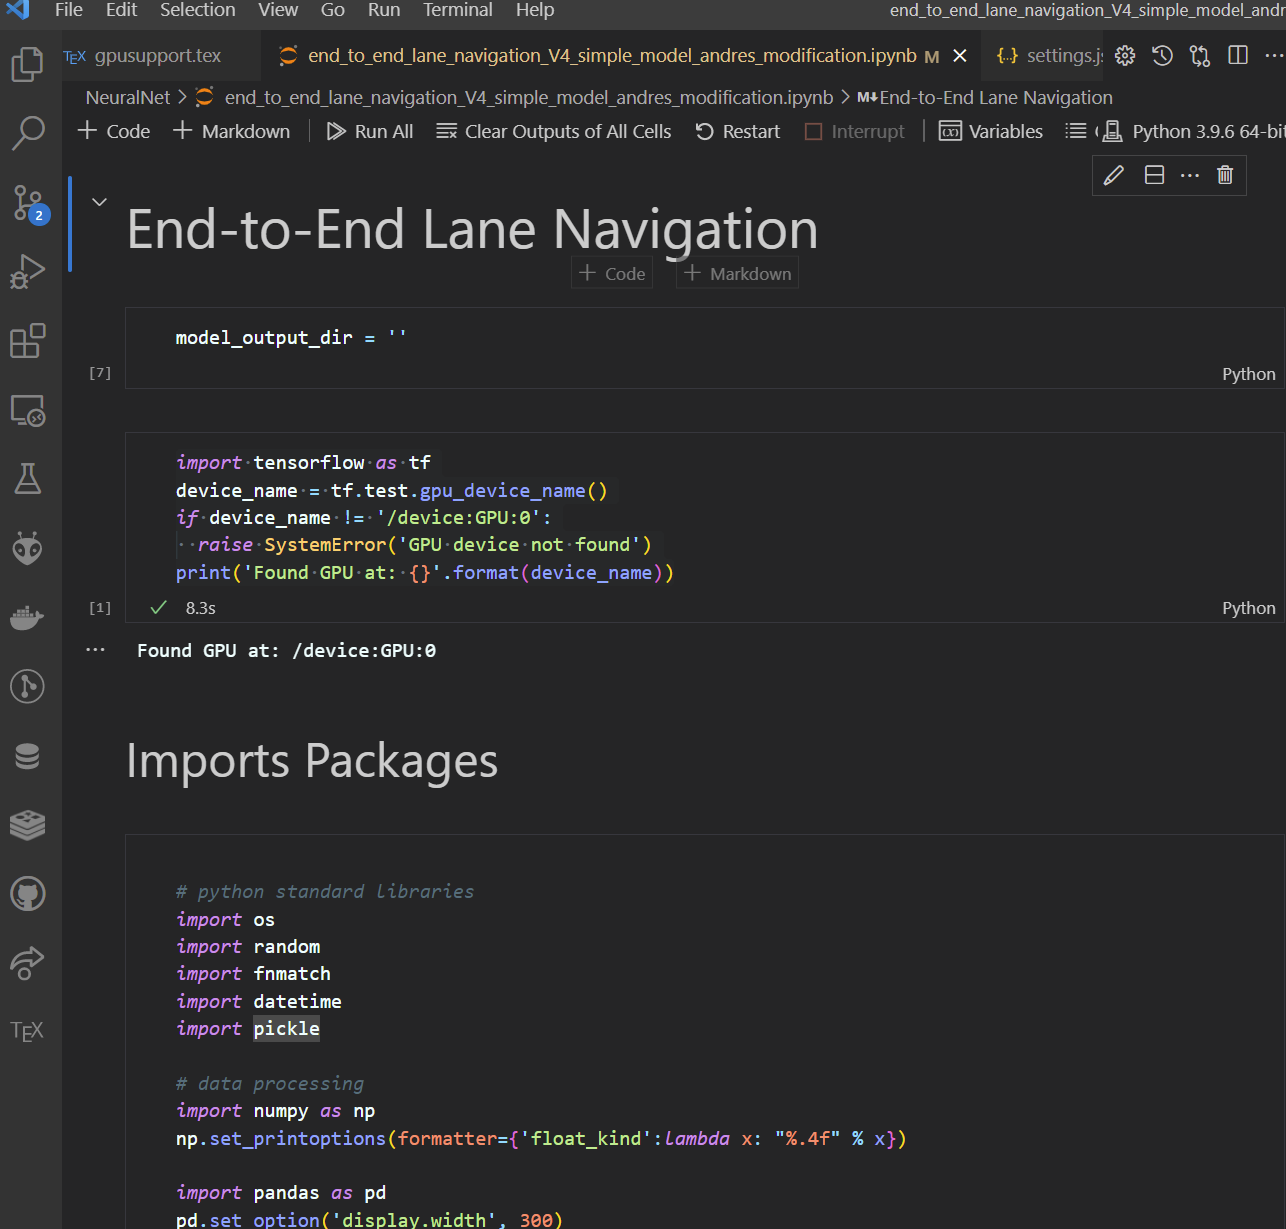
\includegraphics[width=1\textwidth]{final.png}
Your Editor should look something like this. 
\end{center}

\end{document}